\section{Source Code as Trees}\label{SourceCodeAsTrees}
As mentioned in \myref{Chp:CompilerOverview} the compiler parses the source code into a tree.
But before this can be done the source code's symbols is separated into tokens adhering to the \acrshort{cfg} of \gls{gamble}.
These tokens are then further separated into the productions from the \acrshort{cfg}. 
These productions are recursive, and therefore a recursive data structure like a tree is very compatible with the productions.
The tree structure is useful for this purpose because every node of the tree can contain information, and have children and parents which makes it possible to express the productions of a grammar by following a path on the tree from the root to a leaf.
A parse tree, which is the tree a parser produces, separates the source code into different productions of the grammar it represents, but also contains all of the syntax from the grammar, such as parenthesis.
The tree structure makes it possible to traverse the tree in the same path as the source code is written, which means that the tree is not only able to express statements of the source code but also the order in which they are to be executed.
An example of parse tree from the declaration \texttt{int a = 5;} is shown in \myref{image:PST}

\begin{figure}
    \centering
    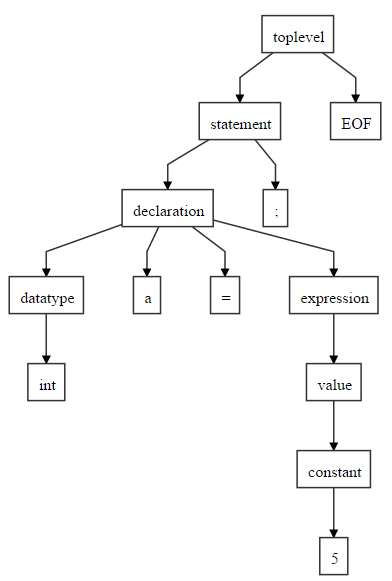
\includegraphics[width=0.5\linewidth]{figures/Trees/PST.PNG}
    \caption{A parse tree from the expression \texttt{int a = 5;} using \glspl{gamble} \acrshort{cfg}.}\label{image:PST}
\end{figure}

The following chapter will explain how the compiler creates a parser to produce these parse trees for the source code, and thus making it possible to use the trees in the compiler.
